\documentclass[14pt, a4paper]{extreport}

\usepackage{geometry}

\usepackage{graphicx}
\graphicspath{{./Images/}}

\usepackage{fontspec}
\usepackage{polyglossia}
\usepackage{hyphenat}

\setotherlanguage{english}

\defaultfontfeatures{Ligatures=TeX}

\setmainfont{Times New Roman}
\setsansfont{Arial}
\setmonofont[Scale=0.8]{DejaVu Sans Mono}

\usepackage{unicode-math}
\setmathfont{Latin Modern Math}

\geometry{
	a4paper,
	left=25mm,
	right=10mm,
	top=15mm,
	bottom=15mm,
}

\usepackage{setspace}
\onehalfspacing

\usepackage{caption}
\usepackage{float}
\usepackage{listings}
\usepackage{xcolor}

\definecolor{codegreen}{rgb}{0,0.6,0}
\definecolor{codegray}{rgb}{0.5,0.5,0.5}
\definecolor{codepurple}{rgb}{0.58,0,0.82}
\definecolor{backcolour}{rgb}{ 0.976, 0.976, 0.976 }

\usepackage{fancyhdr}
\usepackage{hyperref}
\hypersetup{unicode=true, colorlinks=true, linkcolor=black, urlcolor=black}

\pagestyle{fancy}
\fancyhf{}
\renewcommand\headrulewidth{0pt}
\cfoot{\thepage}

\setlength{\headheight}{18pt}

\usepackage{indentfirst}

% Const
\newcommand{\CourseTitle}{Програмування комп'ютерних та віртуальних мереж}
\newcommand{\Variant}{5}
\newcommand{\StudentGroup}{ІМ-51мн}
\newcommand{\CourseNumber}{1}
\newcommand{\StudentName}{Ковальов Олександр}
\newcommand{\Teacher}{доцент, Долголенко Олександр Миколайович}
\newcommand{\Year}{2025}

% Change this
\newcommand{\LabNumber}{1}
\newcommand{\Topic}{Ознайомлення з Mininet}
\newcommand{\SubmissionDate}{24.09.2025}

\lstdefinestyle{mystyle}{
	backgroundcolor=\color{backcolour},   
	commentstyle=\color{codegreen},
	keywordstyle=\color{magenta},
	numberstyle=\tiny\color{codegray},
	stringstyle=\color{codepurple},
	basicstyle=\ttfamily\footnotesize,
	breakatwhitespace=false,         
	breaklines=true,                 
	captionpos=b,                    
	keepspaces=true,                 
	numbers=left,                    
	numbersep=5pt,                  
	showspaces=false,                
	showstringspaces=false,
	showtabs=false,                  
	tabsize=2
}

\lstset{style=mystyle}

\usepackage{enumitem}
\setlist[enumerate]{
	itemsep=0.0\baselineskip,
	left=1.25cm,
	rightmargin=10mm,
	labelsep=0.5cm,
	listparindent=1.25cm,
	parsep=0pt
}

\begin{document}
	
	\begin{titlepage}
		\begin{center}
			{Національний технічний університет України\\
				«Київський політехнічний інститут імені Ігоря Сікорського» \\[1.0em] }
			{Факультет інформатики та обчислювальної техніки\\}
			{Кафедра обчислювальної техніки \\[5.0em]}
			
			{\textbf{ЗВІТ}\\[1em]}
			{\textbf{з лабораторної роботи №\LabNumber} \\}
			{\textbf{з дисципліни "\CourseTitle"} \\[2.0em]}
			
			{\textbf{Тема: \Topic} \\[2.0em]}
			
			{\textbf{Варіант №\Variant} \\[5.0em]}
			
			\begin{flushright}
				Виконав: \\
				Студент \CourseNumber{} курсу, групи \StudentGroup \\
				\StudentName \\[2.0em]
			\end{flushright}
			
			\begin{flushright}
				Перевірив: \\
				\Teacher \\[2.0em]
			\end{flushright}
			
			\begin{flushright}
				Дата здачі: \SubmissionDate \\[5.0em]
			\end{flushright}
		
			\vfill
			КИЇВ -- \Year
		\end{center}
	\end{titlepage}
	
	\setlength{\parindent}{1.25cm}
	
	\textbf{Мета роботи.} Ознайомитись з Mininet - середовищем для моделювання комп'ютерної SDN мережі.
	
	\textbf{Завдання:}
	\begin{enumerate}[noitemsep, nolistsep]
		\item Встановити Mininet;
		\item Створити мінімальну готову топологію SDN мережі;
		\item Продемонструвати (з коментарями) використання основних команд: \texttt{nodes}, \texttt{net}, \texttt{ifconfig}, \texttt{down}, \texttt{up}, \texttt{route}, \texttt{ping}, \texttt{pingall}, \texttt{iperf}, \texttt{ps}, \texttt{xterm}.
	\end{enumerate}
	
	\begin{center}
		\textbf{Хід роботи.}
	\end{center}
	
	Для використання Mininet був встановлений гіпервізор VirtualBox. Після імпортування віртуальної машини, її можна запустити з наданим логіном та паролем. Але, щоб мати змогу підключитися за допомогою протоколу SSH, треба додати "Host-only Network" ресурс. Цей процес продемонстрований на зображенні. Далі, в налаштуваннях віртуальної машини, цей адаптер треба встановити під номером 2, який на системі повинен відображатися як \texttt{eth1}.
	
	\begin{figure}[H]
		\centering
		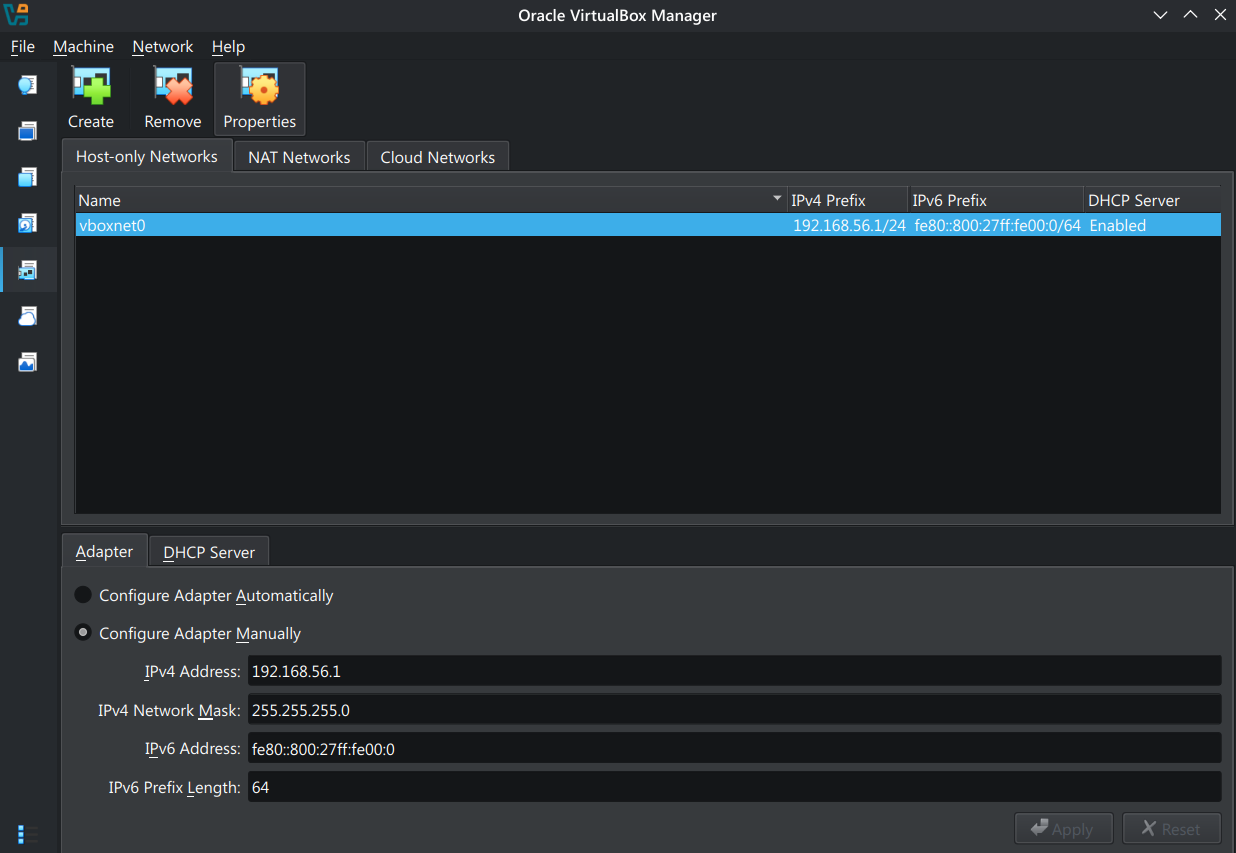
\includegraphics[height=10cm]{01} 
	\end{figure}
	
	Але, скоріш за все, після запуску машини, мережевий інтерфейс не буде встановленим. Для виправлення цієї проблеми треба застосувати команду:
	
	\begin{lstlisting}[language=Bash]
		sudo dhclient eth1\end{lstlisting}
	
	Після чого вже можна встановити зв'язок між хостом та гостьовою машиною.
	Щоб кожного разу не вводити пароль \texttt{mininet} при вході в гостьову систему, бажано додати публічний ключ RSA на сервер. Для цього треба згенерувати ключ якщо його немає, скопіювати на гостьову машину за допомогою утиліти \texttt{scp}, створити файл в якому SSH сервер перевіряє "авторизовані" ключі, надати відповідні права файлам. Всі виконані дії продемонстровані на зображенні.
		
	\begin{figure}[H]
		\centering
		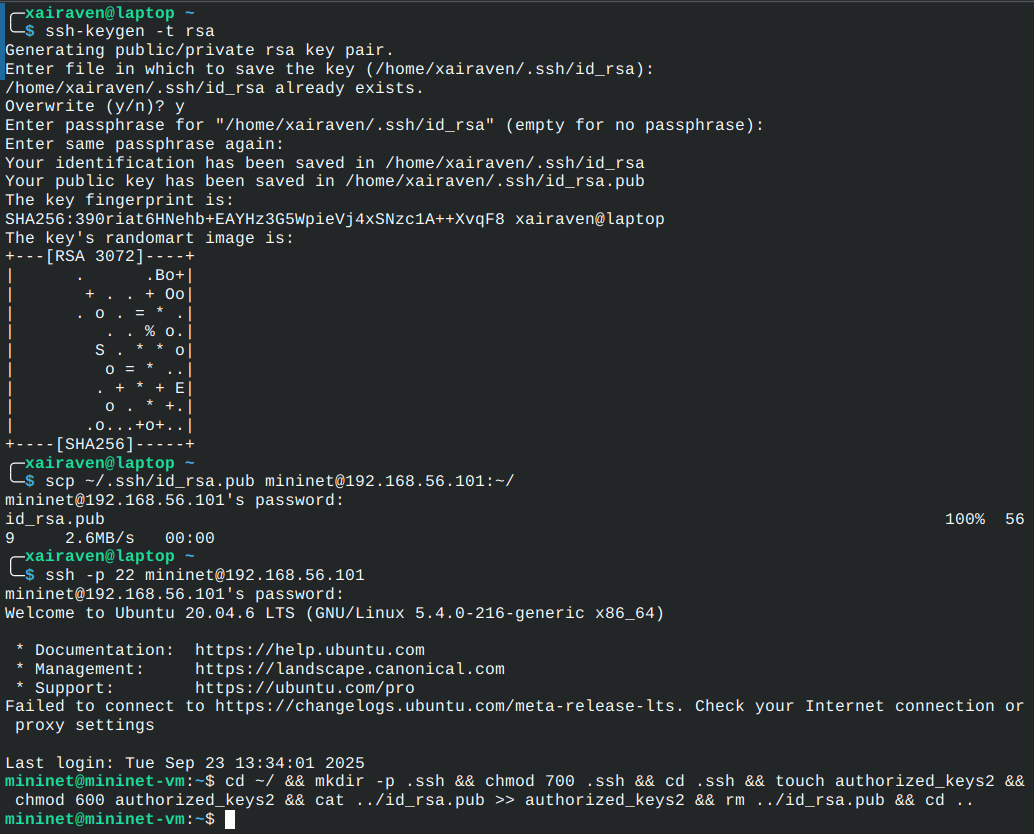
\includegraphics[height=13cm]{02} 
	\end{figure}
	
	Далі, треба запустити Wireshark. Щоб мати змогу користуватись GUI засто\hyp{}сунками через SSH, треба налаштувати X11 тунелінг, де Х11 - віконна система. Щоб все працювало справно, треба щоб на хостовій системі працював Х сервер. Так як лабораторна робота виконується на дистрибутиві Fedora 42 з використанням середовища робочого столу KDE Plasma, де за замовчуванням встановлена сесія протоколу Wayland, треба довстановити потрібні пакети, а саме \texttt{xorg-x11-xauth} та \texttt{xorg-x11-server-Xwayland}. 
	
	\begin{figure}[H]
		\centering
		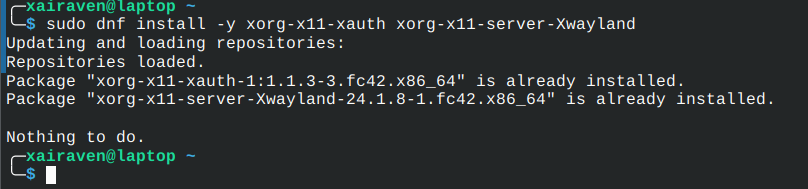
\includegraphics[height=4cm]{03} 
	\end{figure}
	
	Далі, вже на гостьовій машині, треба змінити налаштування SSH серверу, тобто відредагувати файл \texttt{/etc/ssh/sshd\_config}. Якщо потрібних налаштувань стосовно Х11 немає, то треба їх додати.
	
	\begin{figure}[H]
		\centering
		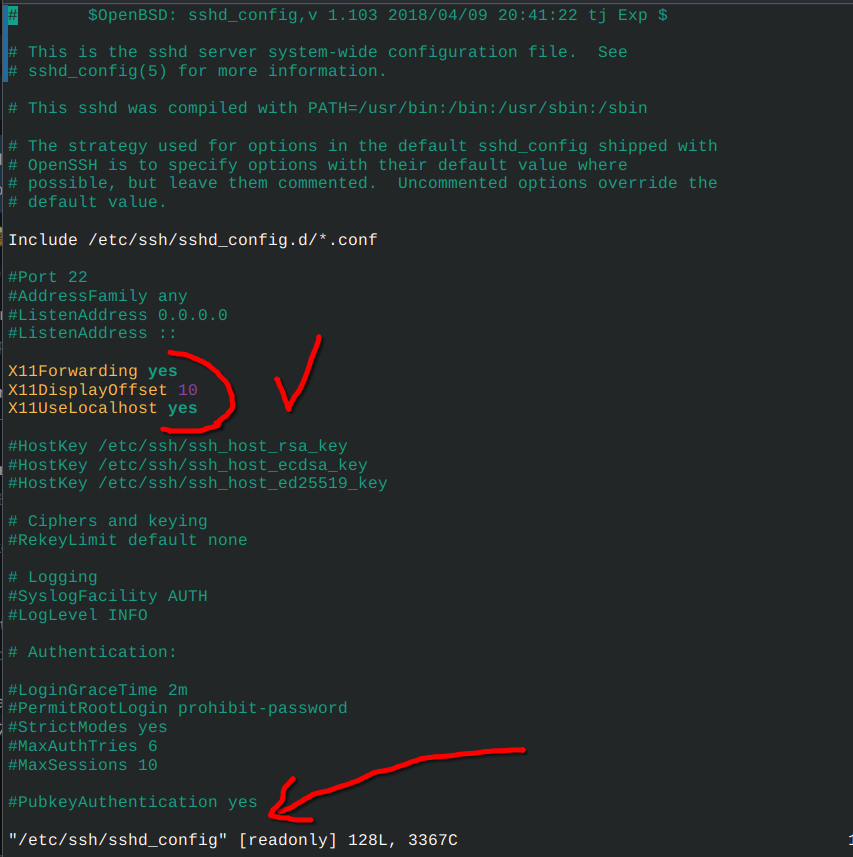
\includegraphics[height=10cm]{04} 
	\end{figure}
	
	Далі, можна перевірити роботу механізму тунелінгу. По-перше, треба підклю\hyp{}читися до гостьової машини використовуючи ключ -X, що дозволяє працювати даному механізму:
	
	\begin{lstlisting}[language=Bash]
		ssh -X -p 22 mininet@192.168.56.101\end{lstlisting}
	
	Для перевірки, можна вивести змінну \texttt{\$DISPLAY} (вказує, куди переводити відображення графічних додатків), або ж запустити додаток \texttt{xclock}.
	
	\begin{figure}[H]
		\centering
		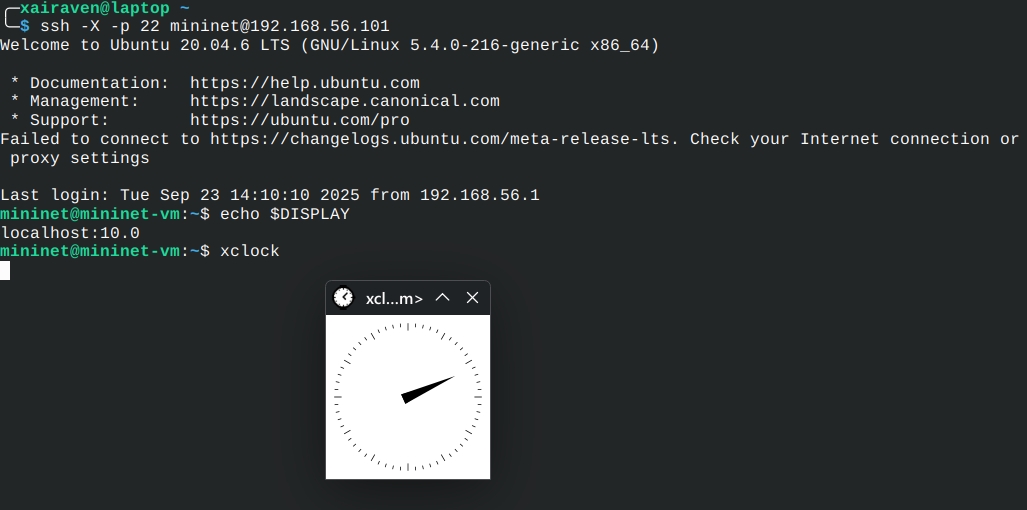
\includegraphics[height=8cm]{05} 
	\end{figure}
	
	Далі можна запустити Wireshark, який успішно запуститься, якщо використати команду \texttt{sudo -E wireshark \&}. Тобто, утиліта запускається у фоні щоб не перекрива\hyp{}ти потік введення, і окремо використовується прапорець -Е, який потрібен щоб при використанні sudo було збережене оточення користувача, а саме вищезазначена змінна \texttt{\$DISPLAY}.
	
	\begin{figure}[H]
		\centering
		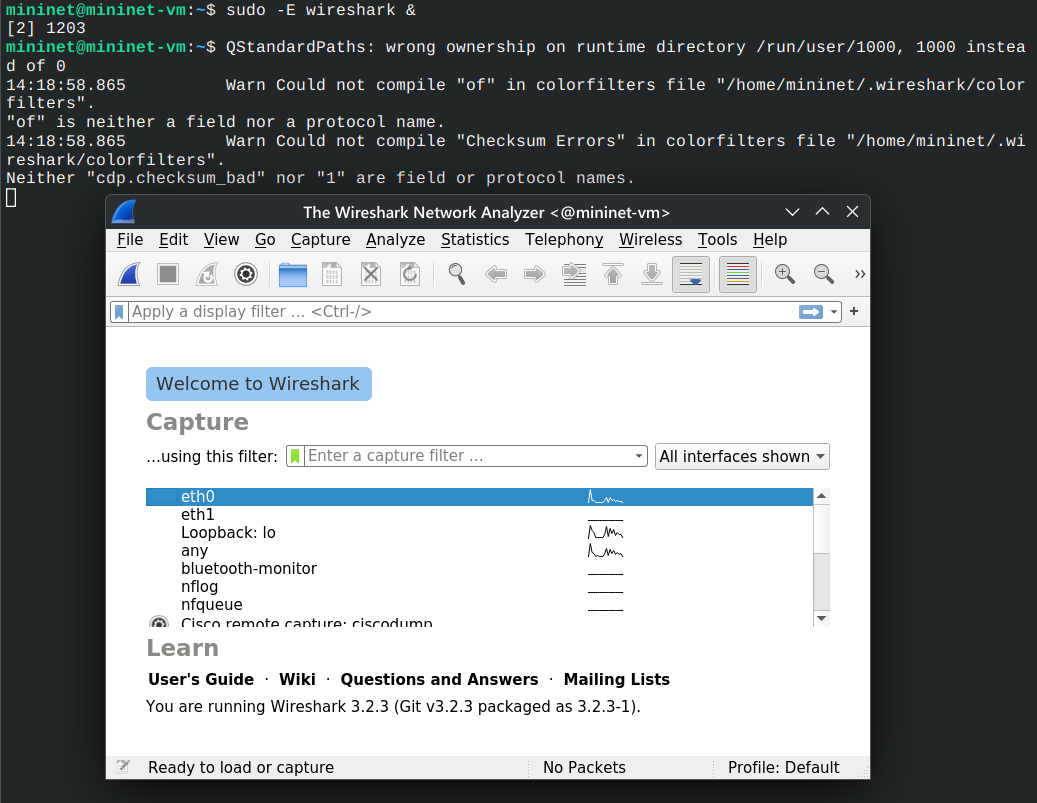
\includegraphics[height=10cm]{06} 
	\end{figure}
	
	Була запущена утиліта \texttt{mininet}, тобто, водночас, була створена мінімальна топологія - OpenFlow контролер, два пристрої та коммутатор.
	
	\begin{figure}[H]
		\centering
		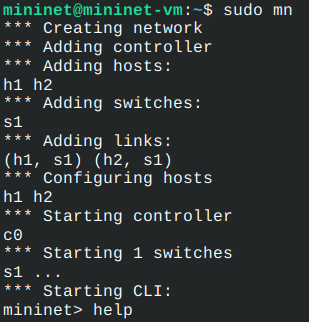
\includegraphics[height=10cm]{07} 
	\end{figure}
	
	Відобразити всі вузли і зв'язки між ними можна відповідно за допомогою команд \texttt{nodes} та \texttt{net}. Можна побачити мінімальну топологію та створені зв'язки: першого хоста зі свічем, другого хоста з ним, та зв'язки комутатора з ними обома.
	
	\begin{figure}[H]
		\centering
		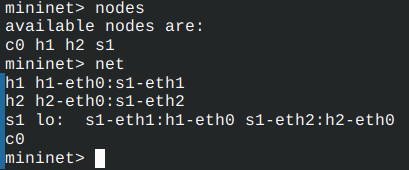
\includegraphics[height=7cm]{08} 
	\end{figure}
	
	Стан мережевих інтерфейсів можна перевірити за допомогою команди \texttt{ifconfig -a}. Відповідно, на зображенні - мережеві інтерфейси двох хостів.
	
	\begin{figure}[H]
		\centering
		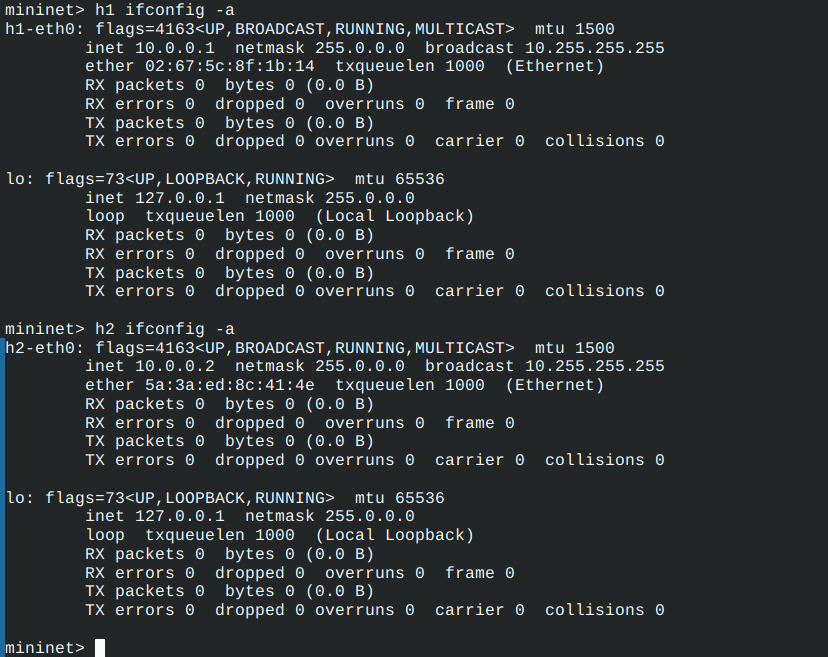
\includegraphics[height=14cm]{09} 
	\end{figure}
	
	Стан комутатора майже повністю співпадає зі станом інтерфейсів системи - це пов'язано з тим, що він працює в просторі імен кореневої мережі.
	
	\begin{figure}[H]
		\centering
		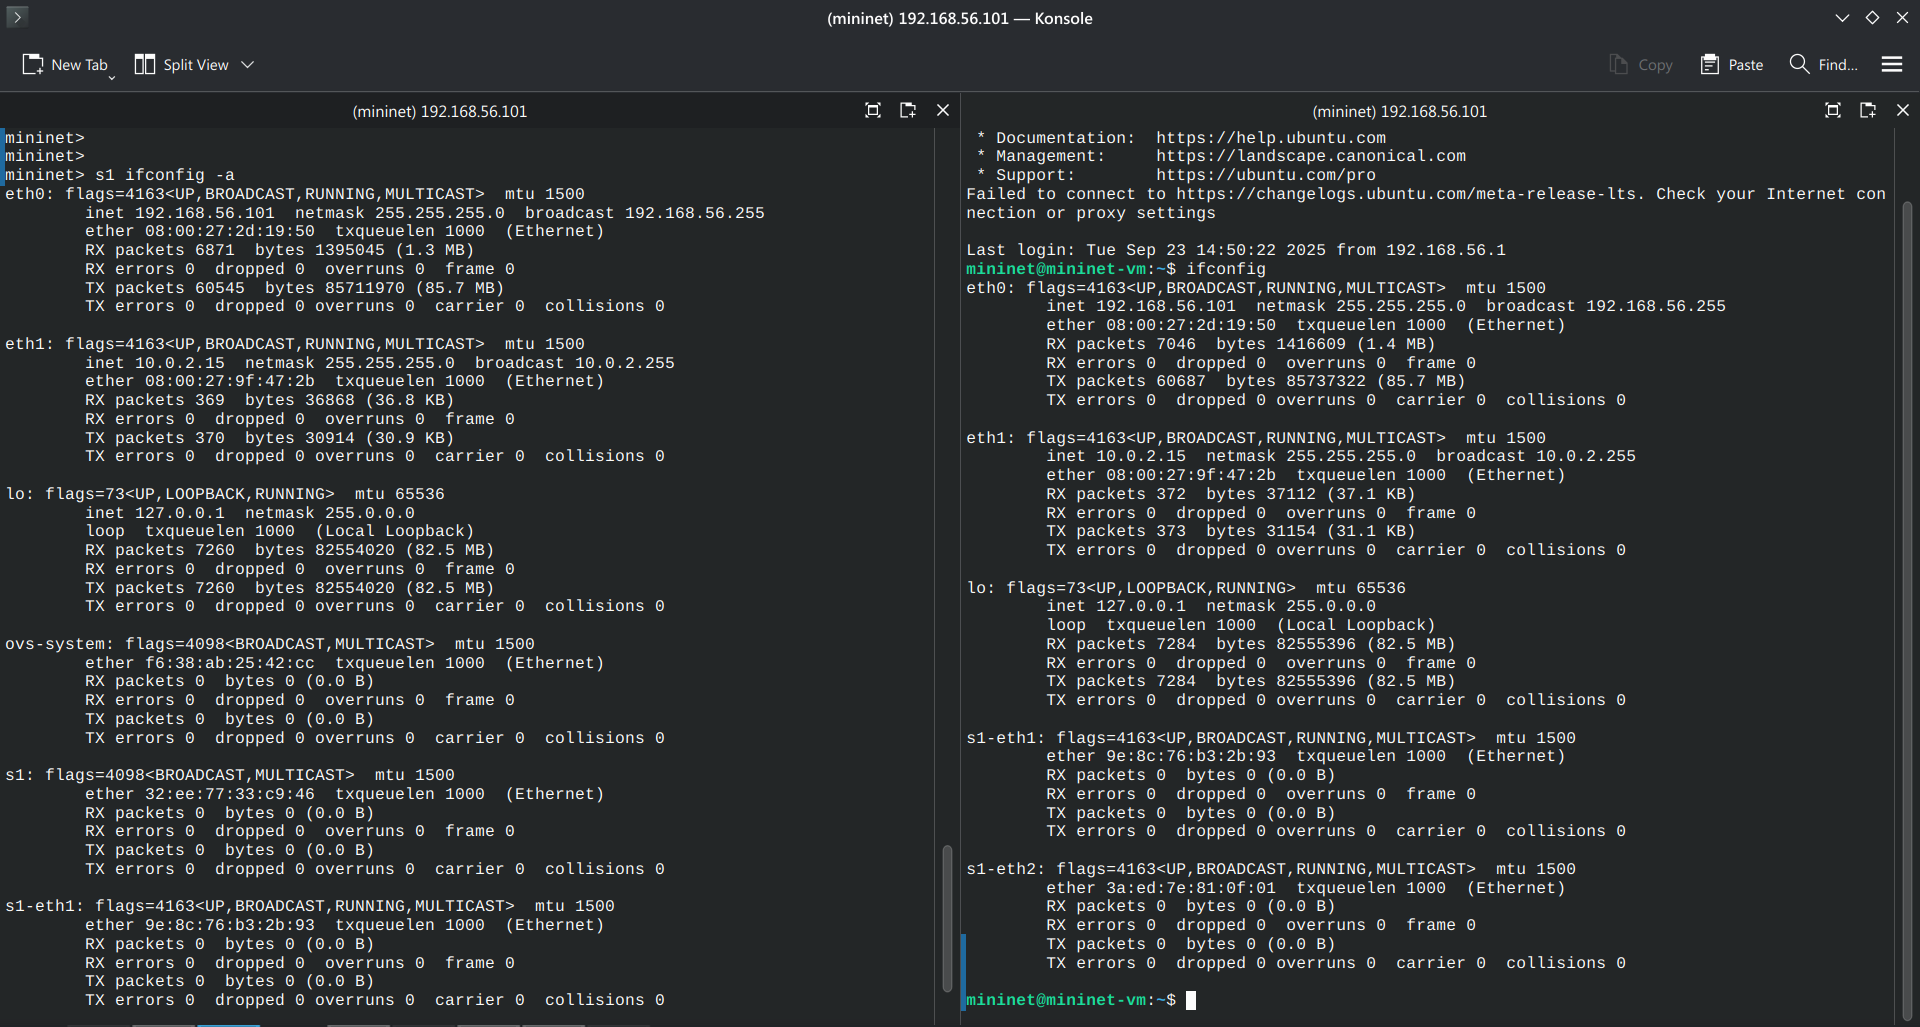
\includegraphics[height=9cm]{10} 
	\end{figure}
	
	Список процесів, запущених на пристрої, можна переглянути використовуючи команду \texttt{ps}.
	
	\begin{figure}[H]
		\centering
		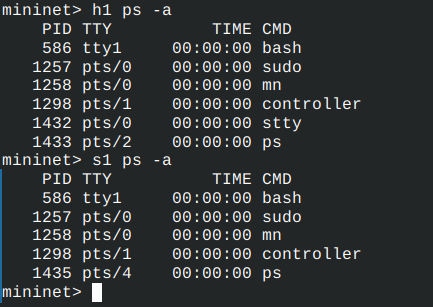
\includegraphics[height=9cm]{11} 
	\end{figure}
	
	Для перевірки доступності вузлів використовується команда \texttt{ping}.
	Перший хост запитує ARP для MAC-адреси другого, що призводить до надсилання повідом\hyp{}лення \texttt{packet\_in} до контролера. Потім контролер надсилає повідомлення \texttt{packet\_out}, щоб переслати широкомовний пакет на інші порти комутатора (у цьому прикладі єдиний інший порт даних). Другий хост бачить ARP-запит і надсилає відповідь. Ця відповідь надходить до контролера, який надсилає її до першого хоста.
	
	Тепер перший хост знає MAC-адресу другого та може надіслати свій \texttt{ping} через ICMP Echo Request. Цей запит разом із відповідною відповіддю від другого хоста надсилається до контролера та призводить до виводу запису потоку (разом із фактичним надсиланням пакетів).

	Видно, що час роботи утиліти набагато менший час для другої спроби. Це відбувається через повторення операції, тобто пакети одразу проходять через кому\hyp{}татор.
	
	Простіший спосіб виконати цей тест - скористатися вбудованою командою \texttt{pingall} в інтерфейсі командного рядка Mininet, яка виконує \texttt{ping} для всіх пар.
	
	\begin{figure}[H]
		\centering
		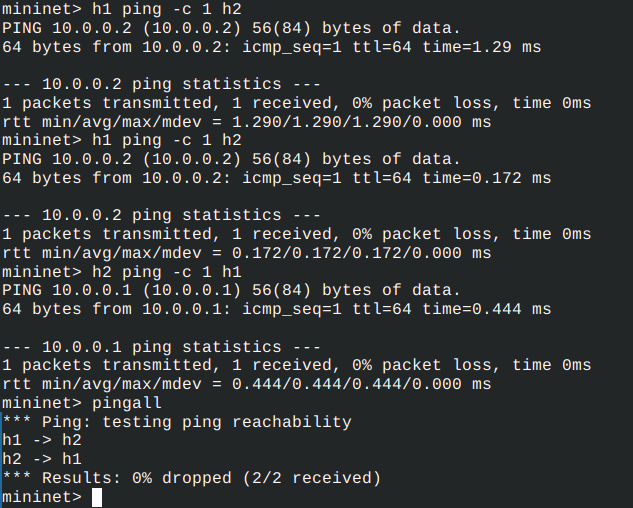
\includegraphics[height=18cm, width=18cm]{12} 
	\end{figure}
	
	Для перевірки пропускної здатності мережі, можна запустити тест за допомогою команди \texttt{iperf}. Це можна зробити і безпосередньо в консолі самої системи, а не застосунку.
	
	\begin{figure}[H]
		\centering
		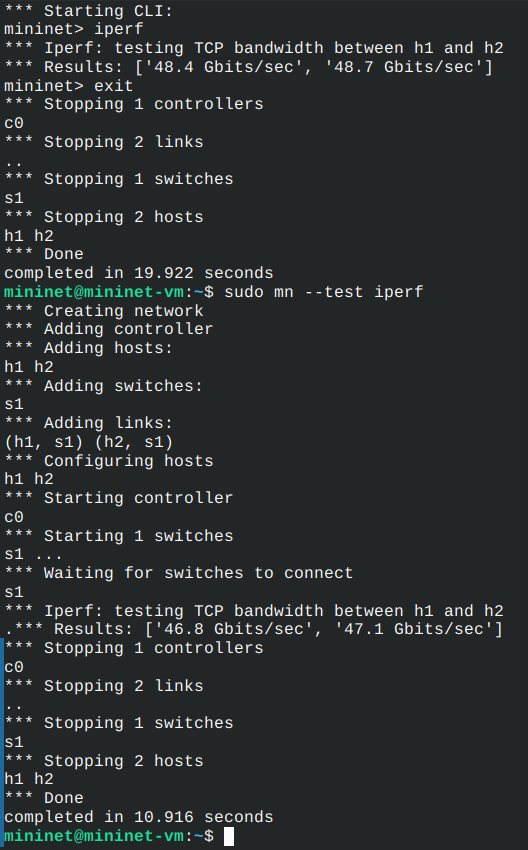
\includegraphics[height=24cm]{13} 
	\end{figure}
	
	Для перегляду або проведення маніпуляцій з таблицею ІР-маршрутизації використовується команда \texttt{route}. Можна помітити, що у комутатора є шлях до інтерфейсу системи - пояснення вже є вище.
	
	\begin{figure}[H]
		\centering
		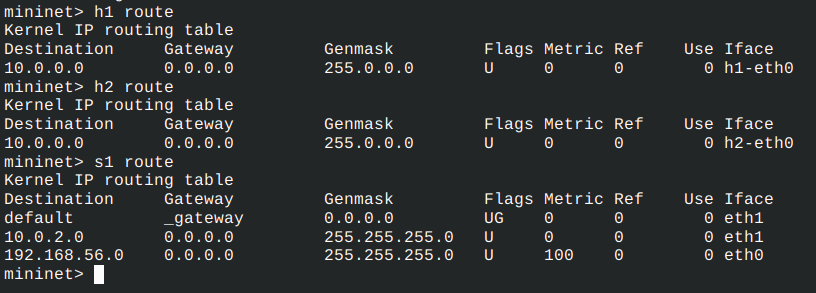
\includegraphics[height=6cm]{14} 
	\end{figure}
	
	Для тестування перенаправлення шляхів чи інших параметрів, можна вмикати або вимикати з'єднання за допомогою команд \texttt{link up} та \texttt{link down}. На зображенні можна спостерігати, що після вимкнення з'єднання не можливо передати ICMP пакет з одного пристрою на інший.
	
	\begin{figure}[H]
		\centering
		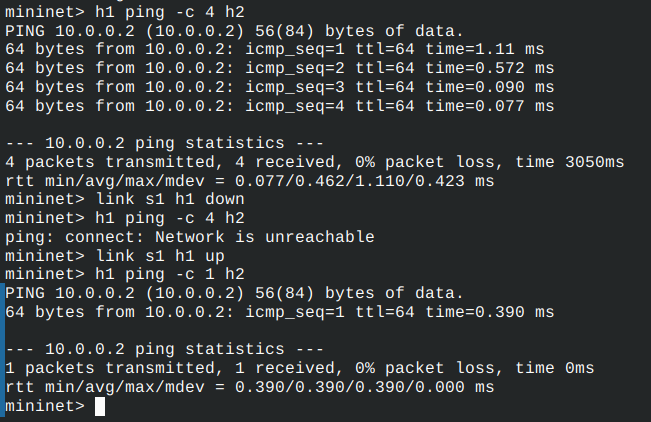
\includegraphics[height=14cm, width=18cm]{15} 
	\end{figure}
	
	Насамкінець, за допомогою Х11-тунелінгу можна запустити термінали прис\hyp{}троїв. Команда \texttt{sudo -E mn -x} дає доступ до всіх терміналів відразу, але можна отримати, наприклад, до двох:
	
	\begin{lstlisting}[language=Bash]
		mininet> xterm h1 h2\end{lstlisting}
	
	На зображенні можна побачити роботу вищезазначеної команди.
	
	\begin{figure}[H]
		\centering
		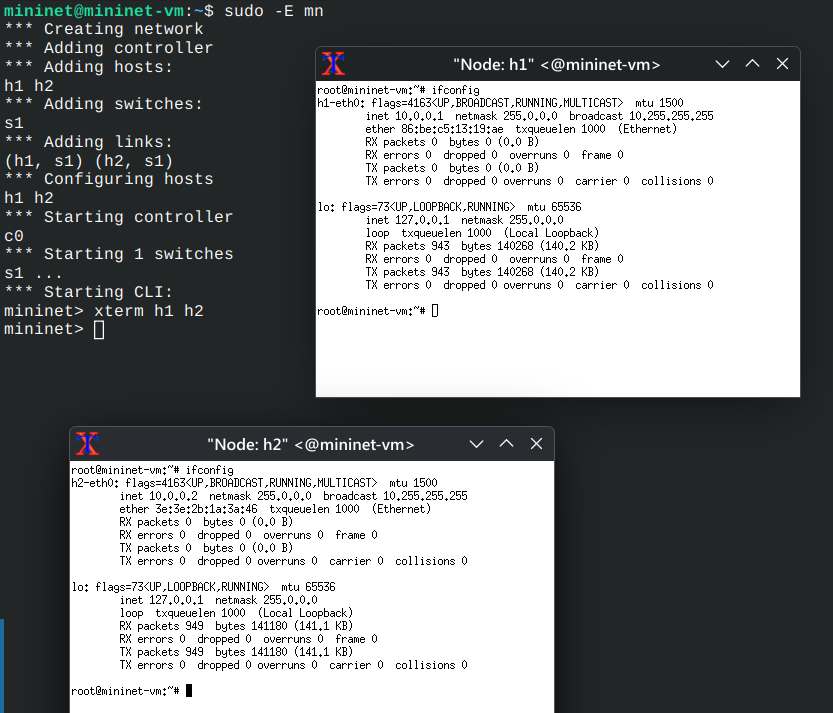
\includegraphics[height=11cm]{16} 
	\end{figure}
	
	\textbf{Висновок.}
	Було ознайомлено з Mininet, зокрема з встановленням віртуальної машини, налаштуванням SSH і X11 та запуском Wireshark.
	Було створено мінімальну топологію та відпрацьовано базові команди (nodes, net, ifconfig, ping, iperf, xterm).
	Було проведено спостереження за обміном через контролер і за поведінкою при link down/up; зроблено висновок, що Mininet ефективний для навчальної симуляції SDN.
	
\end{document}
